\subsection{Descripci\'on del problema}

En este ejercicio se nos presenta el juego Saltos en la Matrix, el mismo se basa en el siguiente reglamento:

\begin{itemize}
\item Se posee un campo de juego cuadrado de N x N celdas.
\item Cada participante comienza en una posici\'on arbitraria $origen$ y debe llegar a la posici\'on $destino$.
\item Para moverse los participantes deber\'an ir saltando por las celdas de manera horizantal o vertical, no as\'i en diagonal.
\item Cada celda posee una potencia $p_{max}$ m\'axima de salto, los participantes podr\'an elegir una potencia $p$ entre 1 y $p_{max}$ para saltar hacia otra celda.
\item A modo de 'bonus' cada jugador posee $k$ unidades extra que podr\'a ir distribuyendo de la manera que desee y las mismas tienen como objetivo otorgarle a los participantes la posiblidad de realizar un salto m\'as potente de lo que la celda le proporciona en caso de creerlo conveniente. Por ejemplo, si un jugador est\'a ubicado en una celda que le posibilita saltar como mucho 2 celdas, pero el mismo considera beneficioso saltar 5, entonces el participante podr\'a utilizar 3 de sus unidades extra para realizar el salto deseado.
\end{itemize}

Como objetivo del ejercicio se nos pide presentar un algoritmo que tome los datos necesarios y devuelva como resultado una secuencia de saltos v\'alida que resuelva el problema en la menor cantidad de saltos posible.

Por otro lado el algoritmo no podr\'a tener una complejidad temporal de peor caso mayor a O($n^3 \cdot k$).

En caso de existir m\'as de una soluci\'on \'optima se podr\'a retornar cualquiera de ellas.


\subsection{Resoluci\'on y demostraci\'on}

Para la resoluci\'on del ejercicio decidimos modelar el tablero con un grafo dirigido sin pesos en sus aristas. Una primera intuici\'on nos llev\'o a asignarle a cada casilla un nodo del grafo y las aristas que parten desde cada nodo representaban los posibles saltos entre casillas. Aunque este enfoque no es del todo incorrecto, no modela correctamente la variable de potencia adicional $k$ que uno posee a lo largo del juego. Si bien uno en una casilla de poder $p$ puede alcanzar las casillas tanto horizontales como verticales a distancia menor o igual a $p$, uno puede aumentar el rango de salto usando la potencia extra $k$. \\

Para poder representar esta informaci\'on en el grafo decidimos que los nodos ademas de representar casillas, representan a las mismas pero en distintos posibles estados. Estos estados pueden ser el no haber gastado ningun $k$ en el momento que se encuentra en esa casilla, o caso contrario cuanto fue gastado para llegar hasta esa casilla a lo largo del camino realizado.

%\begin{figure}[h]
%\begin{center}
%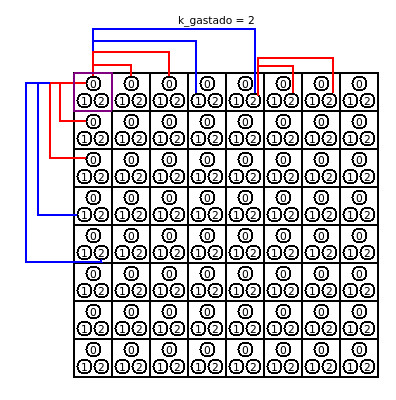
\includegraphics[scale=0.6]{./img/ej3_res1.png}
%\caption{Ejemplo de modelado del grafo. Cada casilla posee k+1 nodos que representan sus posibles estados. En este ejemplo el k = 2 y el poder de salto de la casilla (1,1) marcada en violeta es p = 2. Las lineas rojas representan saltos sin usar unidades extra de potencia y las lineas azules usandolas.}
%\end{center}
%\end{figure}

Si unimos adecuadamente los nodos respetando las condiciones del juego, podremos modelar correctamente el tablero con todas sus condiciones. Luego solo restar\'a buscar el camino m\'inimo entre el nodo que represente la casilla de inicio y alguno de los nodos posibles de la casilla de salida. Las condiciones a respetar son las siguientes:

\begin{itemize}
\item Desde cualquier nodo (en cualquier estado $q$ de gasto de potencias extras) uno puede saltar hasta $p$ casilleros para cualquiera de los cuatro sentidos cardinales. Por ejemplo, desde la casilla (3,6) con poder de salto 2 en un tablero de 7x7, puedo llegar hasta las casillas (3,7), (3,5) y (3,4) horizontalmente y (1,6), (2,6), (4,6) y (5,6) verticalmente. Esto hace que nuestro algoritmo cree una arista entre los nodos que representan la casilla (3,6) y todos los nodos de las casillas que mencionamos anteriormente que representen el mismo estado $q$ de la casilla de origen.
\item Desde cualquier nodo en un estado $q$ de gasto de potencias extras y siendo $k$ el m\'aximo gasto extra posible, puedo saltar $p+(k-q)$ casilleros horizontal y verticalmente. Si el salto que realice supera los $p$ casilleros, el nodo de llegada debe ser el del casillero destino pero en estado igual a $q+k\_gastado$, donde $k\_gastado$ es el poder adicional usado para llegar a esa casilla. Esto garantiza tener una "memoria" de los $k$ utilizados durante uno de los caminos posibles. Notese que en los nodos que representan casillas con $k$ agotados, las unicas aristas posibles son las que solo utilizan la potencia de la casilla y siempre van a nodos que representan casillas sin $k$ restante. No hacer esto haria que el jugador gane unidades de $k$ que no le corresponden.
\end{itemize}

Una vez armado este grafo dirigido que contiene todos los posibles caminos desde todas las casillas (respetando las reglas del juego), solo resta ver cual es el camino con menor cantidad de saltos que logra llegar a la casilla de salida. Cabe destacar que nuestro grafo no es un grafo con pesos, ya que eliminamos ese factor creando aristas con todos los posibles caminos dependiendo el $p$ de la casilla. Este camino minimo lo buscamos con el algoritmo de recorrido de grafos BFS, una de sus utilidades es buscar caminos minimos en grafos sin peso o con todos pesos iguales.


A continuaci\'on se muestran 2 im\'agenes a modo de ejemplo, un tablero, donde los n\'umeros de cada casillero representa la potencia de salto desde ese lugar, y la segunda imagen es un grafo donde se muestra como est\'an unidos los casilleros marcados en azul en la primera. La representaci\'on en el grafo se hace solo con estos tres casilleros para no hacer un grafo totalmente representativo, pero poco entendible.
Para poder interpretar el grafo se debe tener en cuenta la notaci\'on usada:
\begin{itemize}
\item Los nodos en negrita representan los diferentes estados de las casillas pintadas en azul en la primer imagen.
\item En los nodos se ve un valor ($x$,$y$) que representa la posici\'on en el tablero, y un valor $k$ que se identifica con la potencia restante en ese momento.
\item Las aristas presentan un valor $p$ mediante el cual se muestra la potencia (de la casilla) de salto usada, y un valor $k$ que representa la cantidad de unidades extra de potencia que se sumaron en dicho salto.
\end{itemize}

\begin{figure}[h]
\begin{center}
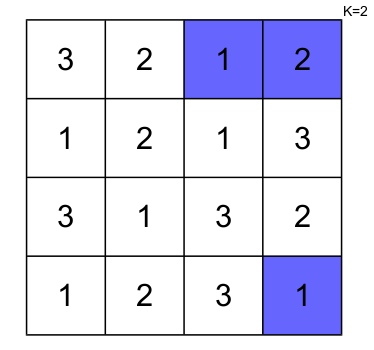
\includegraphics[scale=0.3]{./img/ej3_tablero.png}
\caption{Ejemplo de tablero de juego con k=1}
\end{center}
\end{figure}

\begin{figure}[h]
\begin{center}
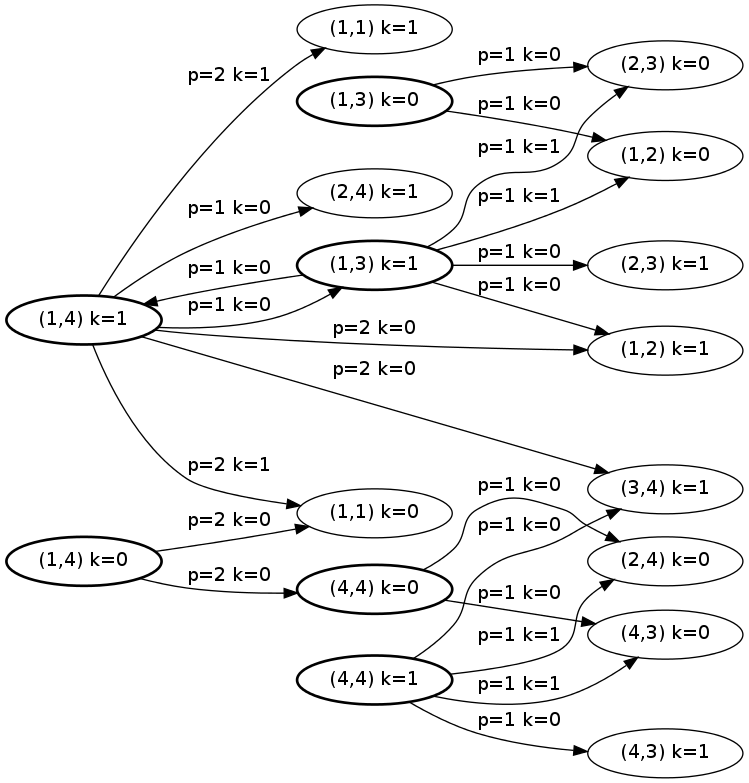
\includegraphics[scale=0.3]{./img/ej3_grafo.png}
\caption{Grafo que representa los posibles saltos entre los casilleros (y estados) pintados en azul en el tablero anterior.}
\end{center}
\end{figure}

Como puede observarse, cada vez que se realiza un salto, si se uso alguna unidad de potencia extra $k$, el salto tiene como destino un nodo que cuenta con la cantidad $k$ restante ($k\_antes\_del\_salto$ - $k\_usado\_en\_el\_salto$), y este a su vez s\'olo tiene aristas hacia nodos con valores $k$ iguales o menores, ya que las unidades no podr\'ian recuperarse.
\newpage
\subsection{Complejidad del algoritmo}

Analizaremos la complejidad del algoritmo propuesto utilizando el siguiente pseudo c\'odigo como gu\'ia:

\begin{itemize}
\item crear una tabla de n*n con las potencias de las casillas, donde $n$ en es el ancho/alto del tablero. (Esto demora exactamente $n^2$ iteraciones)
\item crear un grafo dirigido $G$ de n*n*(k+1) nodos. (Usamos una de listas de adyacencia para representar el grafo. La estructura es un arreglo indexado por el n\'umero de nodo apuntando a punteros de listas. Crear el arreglo cuesta $n^2*(k+1)$ iteraciones, creando una lista vacia en cada iteraci\'on en tiempo constante. \cite{complejidad_lista_construct})
\item para cada nodo $v$ del grafo $G$ (Recorremos los nodos en $n^2*(k+1)$ iteraciones)
	\begin{itemize}
	\item para cada casilla $c$ de la fila del tablero donde se encuentra $v$ (Recorremos las n columnas del tablero, $n$ iteraciones)
		\begin{itemize}
			\item determino si debo unir el nodo $v$ con algun nodo de la casilla $c$ (Esto se realiza en tiempo constante ya que realiza operaciones matem\'aticas y en caso de tener que unirlos agrega un elemento a una lista en tiempo constante \cite{complejidad_lista_push_back})
		\end{itemize}
	\end{itemize}
	\begin{itemize}
	\item para cada casilla $c$ de la columna del tablero donde se encuentra $v$ (Recorremos las n filas del tablero, $n$ iteraciones)
		\begin{itemize}
			\item determino si debo unir el nodo $v$ con algun nodo de la casilla $c$ (Esto se realiza en tiempo constante ya que realiza operaciones matem\'aticas y en caso de tener que unirlos agrega un elemento a una lista en tiempo constante \cite{complejidad_lista_push_back})
		\end{itemize}
	\end{itemize}
\item busco el camino m\'inimo entre la casilla $inicio$ y la casilla $fin$ del grafo $G$ usando BFS ($O(n^3*k)$ (*))
\end{itemize}

(*) El algoritmo BFS tiene una complejidad de O(|V|+|E|), suponiendo el tablero mas denso posible donde se puede ir de cualquier casilla a cualquier casilla (de la misma fila o columna) tenemos $n^2*(k+1)$ nodos y $2*n$ aristas desde cada nodo, resultando $n^3*(k+1)$ aristas. |E| supera a |V| quedando una complejidad de $O(n^3*k)$ \\

Como analizamos, el algoritmo que asigna las aristas de cada uno de los $O(n^2*k)$ nodos se genera con un ciclo que anida 2 ciclos en paralelo de $n$ elementos, completandose toda esta operaci\'on en $O(n^2*k*2*n) = O(n^3*k)$. Finalmente se busca el camino m\'inimo en una complejidad del mismo orden de magnitud.

\newpage
\subsection{C\'odigo fuente}

\lstset{language=C++,
                basicstyle=\ttfamily\footnotesize,
                keywordstyle=\color{blue}\ttfamily,
                stringstyle=\color{red}\ttfamily,
                commentstyle=\color{green}\ttfamily,
                morecomment=[l][\color{magenta}]{\#},
                breaklines=true
}
\begin{lstlisting}
/*
 * Esta funcion decide dados dos nodos si hay una arista entre ellos y de que estado a que estado.
 * Si la hay, agrega la arista al grafo
*/
void unirNodos(directed_graph * grafo, int nro_nodo_fuente, int columna_nodo_fuente, int fila_nodo_fuente, int potencia_nodo_fuente, int estado_nodo_fuente, int columna_nodo_destino, int fila_nodo_destino, bool mirarFila, int tablero_casillas_por_lado, int tablero_k_inicial){
	
	int k_restantes = tablero_k_inicial-estado_nodo_fuente;
	int indice_fuente = 0;
	int indice_destino = 0;
	int nro_nodo_destino = 0;
	
	// Ajustamos los indices que nos interesan segun si estoy recorriendo fila o columna
	if(mirarFila){
		indice_fuente = columna_nodo_fuente;
		indice_destino = columna_nodo_destino;
	}else{
		indice_fuente = fila_nodo_fuente;
		indice_destino = fila_nodo_destino;
	}
	
	// Evito conectar la casilla consigo misma
	if(columna_nodo_fuente != columna_nodo_destino || fila_nodo_fuente!=fila_nodo_destino){
		
		// Verifico si el nodo de destino es alcanzable con la potencia de la casilla actual
		if( ((int) indice_fuente-potencia_nodo_fuente) <= (int) indice_destino && indice_destino <= (indice_fuente+potencia_nodo_fuente)){
			nro_nodo_destino = getNumeroNodo(tablero_casillas_por_lado, tablero_k_inicial, fila_nodo_destino, columna_nodo_destino, estado_nodo_fuente);
			// Conecto el nodo de la casilla actual en estado_nodo_actual 0 con el nodo de la casilla 
			// alcanzable en estado_nodo_actual 0 ya que no gaste ningun k para llegar ahi
			grafo->add_edge(nro_nodo_fuente,nro_nodo_destino);
		
		// Veo si puedo llegar usando k
		}else{
			int diferencia = indice_fuente-(potencia_nodo_fuente+k_restantes);
			
			// Si el poder de la casilla mas los k restantes del estado me lo permiten
			if( diferencia <= (int) indice_destino && indice_destino <= (indice_fuente+potencia_nodo_fuente+k_restantes)){
				int cuanto_k_necesito = 0;
				
				if(indice_fuente <= (int) indice_destino){
					cuanto_k_necesito = indice_destino - potencia_nodo_fuente - indice_fuente;
				}else{
					cuanto_k_necesito = indice_fuente - potencia_nodo_fuente - indice_destino;
				}
				// Lo voy a juntar con el nodo que puedo llegar pero a un estado correspondiente
				nro_nodo_destino = getNumeroNodo(tablero_casillas_por_lado, tablero_k_inicial, fila_nodo_destino, columna_nodo_destino, estado_nodo_fuente+cuanto_k_necesito);
				// Conecto el nodo de la casilla actual en estado_nodo_actual 0 con el nodo de la casilla 
				// alcanzable a su estado_nodo_actual correspondiente segun el gasto de k
				grafo->add_edge(nro_nodo_fuente,nro_nodo_destino);
			}
			
		}
	}
}

\end{lstlisting}

\newpage

\lstset{language=C++,
                basicstyle=\ttfamily\footnotesize,
                keywordstyle=\color{blue}\ttfamily,
                stringstyle=\color{red}\ttfamily,
                commentstyle=\color{green}\ttfamily,
                morecomment=[l][\color{magenta}]{\#},
                breaklines=true
}
\begin{lstlisting}

/*
 * Funcion que dada una fila, una columna y un estado de consumo de k, devuelve el numero de nodo correspondiente
 */
unsigned int getNumeroNodo(unsigned int tablero_casilleros_lado, unsigned int tablero_k, unsigned int fila, unsigned int col, unsigned int estado){
	
	unsigned int nro_nodo = (fila*tablero_casilleros_lado*(tablero_k+1) + (col*(tablero_k+1)) + estado);
	assert(0 <= nro_nodo);
	assert(nro_nodo < tablero_casilleros_lado*tablero_casilleros_lado*(tablero_k+1));
					
	return nro_nodo;
}
/*****************************/
/* CODIGO PRINCIPAL DEL MAIN */
/*****************************/

directed_graph * grafo = new directed_graph(cant_nodos);
		
unsigned int fila_nodo_fuente;
unsigned int columna_nodo_fuente;
unsigned int estado_nodo_fuente;
unsigned int potencia_nodo_fuente;

// Asigno las posibles aristas, i = todos los posibles nodos que representan tanto casillas sin gastos de k como con algun gasto
for(unsigned int nro_nodo_fuente = 0; nro_nodo_fuente<cant_nodos; nro_nodo_fuente++){
	
	// Datos de la casilla fuente
	fila_nodo_fuente = (nro_nodo_fuente / (k+1)) / n;
	columna_nodo_fuente = ((nro_nodo_fuente / (k+1)) % n);
	estado_nodo_fuente = nro_nodo_fuente % (k+1);
	potencia_nodo_fuente = (*potencias)[fila_nodo_fuente][columna_nodo_fuente];
					
	// Recorro la fila y conecto la casilla con todas las alcanzables de la misma
	for(unsigned int columna_nodo_destino=0; columna_nodo_destino<n; columna_nodo_destino++){
		
		int fila_nodo_destino = fila_nodo_fuente;
		
		// Si corresponde, se unen el nodo_fuente con el nodo_destino
		unirNodos(grafo, nro_nodo_fuente, columna_nodo_fuente, fila_nodo_fuente, potencia_nodo_fuente, estado_nodo_fuente, columna_nodo_destino, fila_nodo_destino, true, n, k);

	}
	// Recorro la columna y conecto la casilla con todas las alcanzables de la misma
	for(unsigned int fila_nodo_destino=0; fila_nodo_destino<n; fila_nodo_destino++){
		
		int columna_nodo_destino = columna_nodo_fuente;
		
		// Si corresponde, se unen el nodo_fuente con el nodo_destino
		unirNodos(grafo, nro_nodo_fuente, columna_nodo_fuente, fila_nodo_fuente, potencia_nodo_fuente, estado_nodo_fuente, columna_nodo_destino, fila_nodo_destino, false, n, k);
		
	}
}

\end{lstlisting}

\newpage
\subsection{Casos de prueba}

Incorporamos entre los archivos adjuntos, en TP:/ej3/input/, varios casos de prueba, entre ellos algunos casos borde y otros triviales para comprobar la correctitud del algoritmo.

\begin{itemize}
\item input\_corto: El tablero esta dispuesto de tal forma que desde el casillero inicial se puede llegar en dos saltos al final sin tener que usar unidades extras de potencia.
\item input\_largo: El caso opuesto al anterior, no hay unidades de potencia extra y todos los casilleros tienen el minimo de potencia. Todos los caminos posibles son igual de largos.
\item input\_camino: Para lograr tomar el camino mas corto en este tablero se debe administrar bien las potencias extras ya que a cada salto debe usarse una \'unica unidad de la misma.
\end{itemize}

\subsection{Performance}

Para el an\'alisis de performance de este ejercicio decidimos ejecutar lotes aleatorios de tests siguiendo los siguientes criterios:

Con $n$ = casillas por lado, $k$ = saltos extra

\begin{itemize}
	\item Iteramos $n$ entre 25 y 80 casillas.
	\item En cada iteraci\'on incrementamos la cantidad de casillas en 1 unidad.
	\item Generamos un input con potencias de saltos aleatorios de entre 1 y $n$.
	\item Para cada valor de $n$ iteramos $k$, saltos extra, entre 0 y $n$:
\end{itemize}

Para realizar esto generamos dos scripts de bash:
\begin{itemize}
	\item generador\_inputs.sh
	\item tests.sh
\end{itemize}

El segundo script, tests.sh, es quien se encarga de iterar los valores de $n$ y $k$, para luego, generando inputs mediante la invocaci\'on del otro script, invocar al programa e ir guardando los tiempos de ejecuci\'on para cada valor de $n$ y $k$.

En cuanto a los valores de $n$ y $k$ elegidos cabe comentar la idea planteada: En un comienzo nuestro objetivo era poder experimentar con valores para la cantidad de casillas por lado de 1 al mayor que podamos ejecutar (en un tiempo razonable de algunas horas con computadoras hogare\~nas), pero para valores de $n$ inferiores a 25 la funcionalidad 'clock()' de $c++$ nos devolv\'ia un tiempo de ejecuci\'on igual a cero, por ende para representar gr\'aficamente los resultados debimos comenzar con $n=25$ y finalizar con $n=80$. 
	Para los valores de $k$, los saltos extra, nos pareci\'o interesante ver que pasaba si lo iterabamos entre 0 y $n$ ya que la complejidad tambi\'en depende de los valores que vaya tomando dicha variable.

A la hora de gr\'aficar entendimos que para poder apreciar mejor el comportamiento asint\'otico de los resultados iba a ser necesario normalizar los valores, en nuestro caso lo que realizamos fue dividir los tiempos obtenidos por el valor de $k$ en cada respectiva ejecuci\'on. De esta manera podemos representar los tiempos obtenidos en funci\'on de $n$.

\newpage

\begin{center}
\begin{figure}[h!]
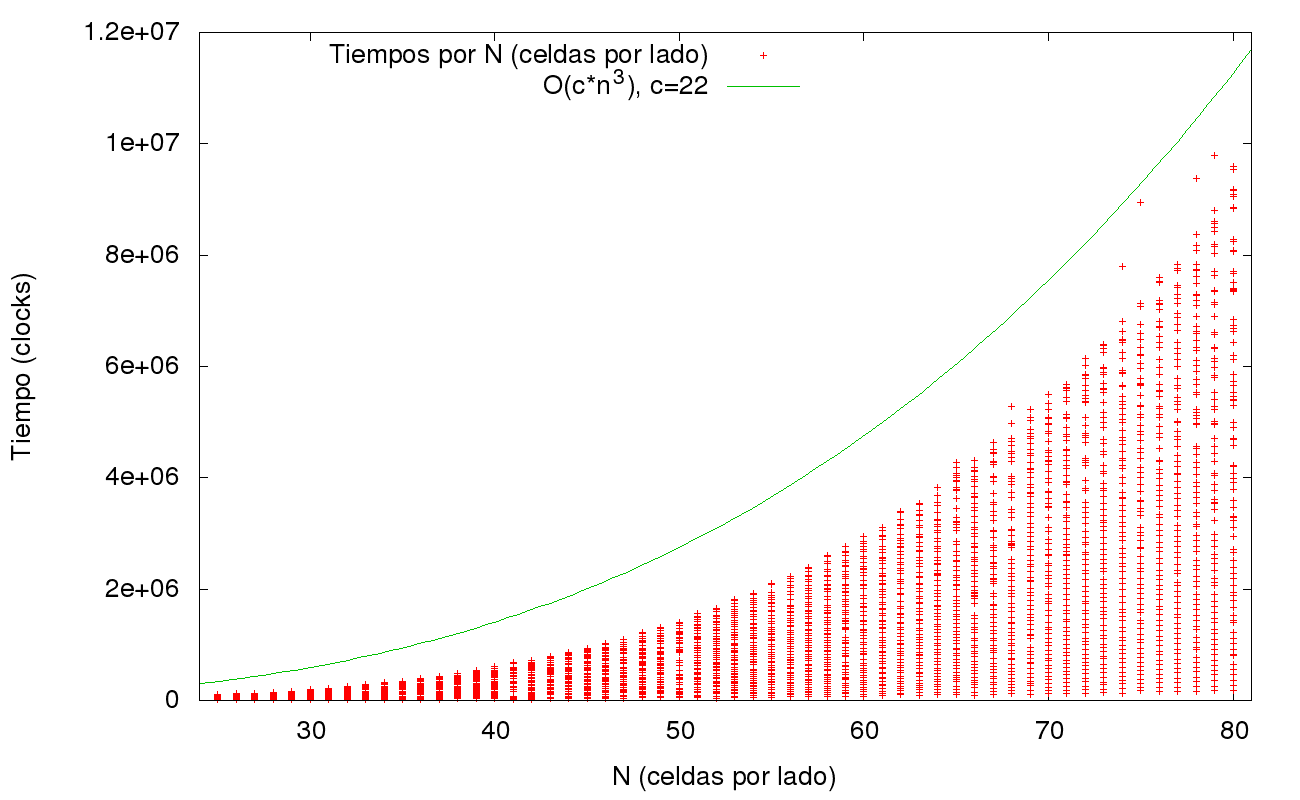
\includegraphics[scale=0.4]{./img/ej3_chart_normalizado.png}
\caption{Tiempo transcurrido por cantidad de casillas por lado (gr\'afico normalizado por $k$)}
\end{figure}
\end{center}


Para poder analizar el comportamiento asint\'otico de los resultados obtenidos gr\'aficamente fue necerio graficar, junto a los tiempos, la funci\'on $c*n^3$, con $c$ una constante, ya que dicha funci\'on es nuestra cota superior.
En cuanto a la b\'usqueda de la constante $c$ simplemente tomamos cada tiempo resultante y lo dividimos por su $n$ de input elevado al cubo, luego, de entre todos los valores calculados tomamos el m\'as grande y de esta manera pudimos ajustar ambos gr\'aficos de manera tal que se pueda visualizar correctamente los resultados.

Como podemos observar, efectivamente los resultados obtenidos se comportan asint\'oticamente de manera correcta ya que su aspecto se asemeja a la funci\'in $n^3$ para los diversos valores de $n$.


Por otro lado, sabiendo que el comportamiento depende de $n$ y $k$, quisimos visualizar para que valores de dichas variables el programa ten\'ia un mejor comportamiento, o, dicho de otra manera, en que momento ibamos a poder encontrar los 'mejores casos'.

Para poder realizar esto fue necesario representar los tiempos obtenidos en funci\'on la cantidad de casillas por lado y de los saltos extra, es decir, en funci\'on de $n$ y $k$. 

\newpage

\begin{center}
\begin{figure}[h!]
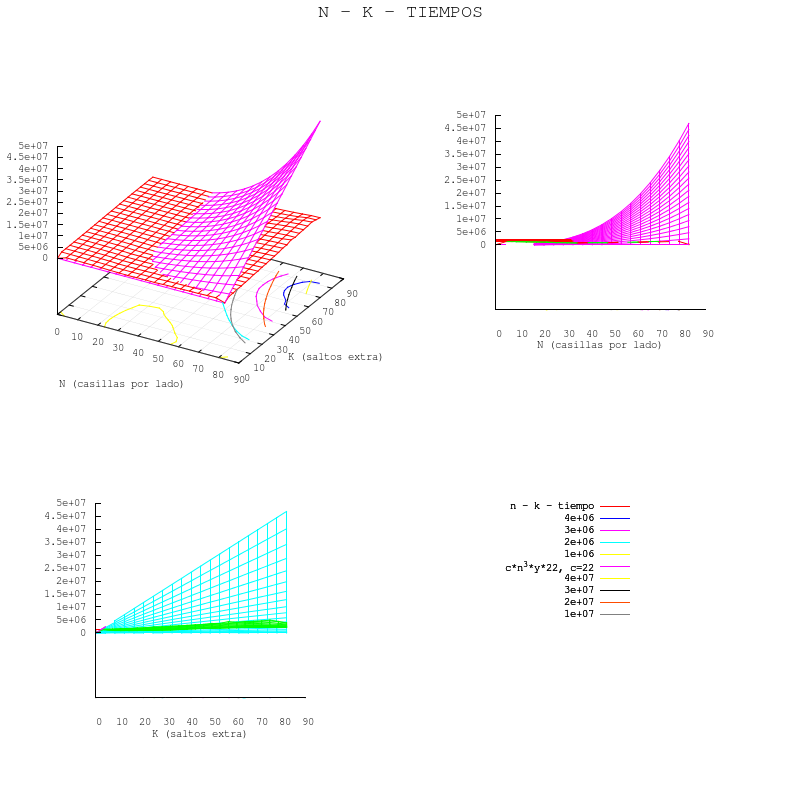
\includegraphics[scale=0.7]{./img/ej3_n_k_tiempos.png}
\caption{Tiempo transcurrido por cantidad de casillas por lado y saltos extrar)}
\end{figure}
\end{center}


Nuevamente utilizamos la constante $c$ calculada previamente para ajustar los resultados a la cota superior.

Como podemos observar, a medida que $n$ y $k$ crecen los resultados se van despegando cada vez m\'as de la cota superior, por lo que el mejor comportamiento lo vamos encontrando a medida que se van incrementando ambas variables de las cuales depende la complejidad, o sea, las casillas por lado y la cantidad de saltos extra.
